% !TeX root=main.tex
\chapter{انتخاب \lr{API}مناسب برای ایجاد ارتباط \lr{Peer to Peer}}
\thispagestyle{empty}

اولین گام برای ساخت یک شبکه‌ی محلی این است که یک 
\lr{API}
موجود یا فناوری موجود را که ارتباط محلی و 
\lr{Peer to Peer}
را برای ما بوجود بیاورد را پیدا کنیم و یا این که از ابتدا قابلیت‌های مورد نیاز را پیاده‌سازی کنیم. بدین منظور چندین 
\lr{API}
شامل
\lr{p2pkit}
\cite{p2pkit}
،
\lr{Alljoyn}
\cite{Alljoyn}
،
\lr{Nearby}
\cite{Nearby}
،
\lr{Hypelabs}
\cite{Hypelabs}
و
\lr{Open Garden}
\cite{OpenGarden} 
را پیدا کردیم.
با این که هر کدام از این 
\lr{API}
ها قابلیت‌های مورد نیاز و اولیه‌ی شبکه‌های اجتماعی را در بردارند، اما مشکل اساسی همه‌ی این 
\lr{API}
ها این است که اپلیکیشنی که بر مبنای این‌ها پیاده‌سازی شده‌باشد، باید به اینترنت متصل باشد تا API بتواند به درستی کار کند. بنابراین از آن جایی که شبکه‌ی اجتماعی ما قرار است بدون اینترنت کار کند، نمی‌توانیم از این 
\lr{API}
ها بهره ببریم.

در ادامه، با فناوری
\lr{WiFi Direct}
 آشنا می‌شویم که بر روی گوشی‌های اندروید موجود است و تمامی قابلیت‌هایی که ما برای برقراری ارتباط محلی گوشی‌ها به یکدیگر را نیاز داریم؛ در خود دارد. با این تفاوت که مشکل 
\lr{API}
ها را هم ندارد و بدون نیاز به اتصال اینترنت می‌تواند کار کند. در ادامه‌ی این فصل به معرفی این فناوری و قابلیت و مزایای آن می‌پردازیم.

\section{فناوری \lr{WiFi Direct}} 
\lr{WiFi Direct}
 فناوری جدید تعریف شده توسط اتحادیه 
\lr{WiFi}
\LTRfootnote{WiFi alliance}
  است که هدف آن ارتقاء ارتباط مستقیم بین دستگاه‌ها است؛ بدون این که به یک نقطه دسترسی بی‌سیم
\LTRfootnote{wireless access point} 
   نیاز باشد.
\lr{WiFi Direct}
بر روی زیر ساخت موفق 
\lr{IEEE 802.11}
بنا شده است و این اجازه را به دستگاه‌ها می‌دهد که در یک ارتباط، یک دستگاه نقش  نقطه دسترسی بی‌سیم را ایفا کند و عملکرد آن را انجام دهد. در حال حاضر می‌توان با استفاده از استاندارد 
\lr{IEEE 802.11}
یک ارتباط مستقیم بین دستگاه‌ها ایجاد کرد. اما اشکالات فراوانی همچون مصرف زیاد انرژی در دستگاه وجود دارد.
\cite{WiFiAlliance}
 
\section{بررسی فنی}
 در یک شبکه معمولی 
\lr{WiFi}
مشتری
\LTRfootnote{client}
 اسکن می‌کند وعضو یکی از شبکه‌های بی‌سیم موجود که توسط نقطه دسترسی بی‌سیم ایجاد و اعلام شده‌است؛ می‌شود. این فرایند در 
\lr{WiFi Direct}
به صورت پویا
\LTRfootnote{dynamic}
انجام می‌شود از این رو یک دستگاه 
\lr{WiFi Direct}
باید هر دو نقش مشتری و نقطه دسترسی بی‌سیم را به طور همزمان اجرا کند.
\cite{WiFiAlliance}

\section{معماری}
دستگاه‌های دارای 
\lr{WiFi Direct}
با ایجاد یک گروه با عنوان 
\lr{P2P Group}
می‌توانند با یکدیگر ارتباط برقرار کنند. دستگاهی که عملکردی همچون نقطه‌ی دسترسی بی‌سیم دارد را 
\lr{P2P Group Owner}
می‌نامند و دستگاهی که در نقش مشتری است را 
\lr{P2P client}
گویند.
هنگامی که یک 
\lr{P2P Group}
ایجاد می‌شود، سایر مشتری‌ها می‌توانند با همان روش سنتی شبکه‌های 
\lr{WiFi}
به گروه بپیوندند. زمانی که یک دستگاه هم در نقش 
\lr{P2P Client}
 و هم در نقش 
\lr{P2P Group Owner}
باشد، دستگاه به طور متناوب با استفاده از اشتراک زمانی 
\LTRfootnote{Time sharing}
بین این دو نقش تغییر می‌کند.(مثال: لپتاپ 2 در بالای شکل \ref{fig:WifiDirectArchitecture})
\cite{WiFiAlliance}

 مانند یک نقطه‌ی دسترسی بی سیم سنتی، یک
\lr{P2P Group Owner}
، خود را از طریق 
\lr{beacons}
  اعلام می‌کند. تنها دستگاهی که 
\lr{P2P Group Owner}
 است؛ قادر است دستگاه‌های متصل در گروه خود را به یک شبکه‌ی خارجی متصل کند.(مثال: موبایل موجود در بالا‌ی شکل \ref{fig:WifiDirectArchitecture}) این ارتباط باید در لایه‌ی شبکه 
\LTRfootnote{Network Layer}
اتفاق بیفتد و معمولا با استفاده از 
\lr{NAT}
\LTRfootnote{Network Address Translation}
پیاده سازی می‌شود.
\lr{WiFi Direct}
اجازه نمی‌دهد که نقش 
\lr{P2P Group Owner}
به افراد دیگری در گروه انتقال یابد.

\begin{figure}
	\centerline{
	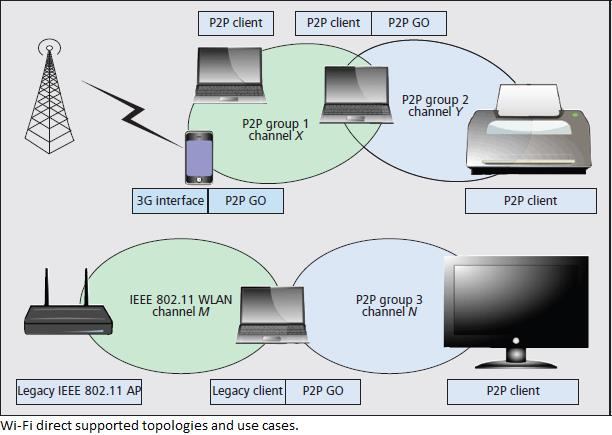
\includegraphics{images/wifidirectarchitecture.jpg}}
	\caption{معماری \lr{Wifi Direct}\cite{Camps-Mur}}
	\label{fig:WifiDirectArchitecture}
\end{figure}

\section{تشکیل گروه}
سه نوع روش برای تشکیل گروه در فناوری
\lr{WiFi Direct}
وجود دارد که عبارتند از استاندار
\LTRfootnote{Standard}
،مستقل
\LTRfootnote{Autonomus}
و پایدار
\LTRfootnote{Persistent}
.

تشکیل گروه شامل دو مرحله است:
\begin{enumerate}
	\item تعیین \lr{P2P Group Owner}
	\begin{itemize}
		\item  دو دستگاه با توجه به تمایل یا قابلیت برای \lr{P2P Group Owner} شدن با یکدیگر مذاکره می‌کنند.
		\item در نهایت در این مرحله نقش مالک گروه در سطح اپلیکیشن ایجاد می‌شود. 
	\end{itemize}
	\item تهیه ی \lr{P2P Group}
	\begin{itemize}
		\item ایجاد \lr{session} گروه با استفاده از مدارک\LTRfootnote{Credentials} معتبر
		\item استفاده از پیکربندی\LTRfootnote{Configuartion} ساده \lr{Wifi} برای تبادل مدارک.
	\end{itemize}
\end{enumerate}

\subsection{استاندارد}\label{subsec:Standard}
در این حالت دستگاه‌ها باید یکدیگر را پیدا 
\LTRfootnote{Discovery}
کنند و سپس مذاکره کنند که کدام دستگاه به عنوان  مالک گروه عمل خواهد کرد. شروع آن با انجام یک اسکن مانند 
\lr{WiFi}
 سنتی است که با استفاده از آن می‌توانند گروه‌ها و شبکه‌های
 \lr{WiFi}
  موجود را پیدا کنند. برای جلوگیری از تضاد، زمانی که دو دستگاه آمادگی خود را برای مالک گروه شدن اعلام می‌کنند، یک بیت 
\lr{tie-breaker}
   در درخواست قرار می‌گیرد. هر بار که یک درخواست ارسال می‌شود، به طور تصادفی این بیت تنظیم می‌شود.
\cite{Camps-Mur}
\subsection{مستقل}
یک دستگاه می‌تواند به صورت خودکار یک گروه  ایجاد کند و بلافاصله این دستگاه مالک گروه می‌شود. دستگاه‌های دیگر می‌توانند گروه‌های ایجاد شده را با استفاده از مکانیزم‌های سنتی اسکن پیدا کنند. در مقایسه با بخش \ref{subsec:Standard}، مرحله پیدا کردن در این مورد ساده تر است، زیرا مرحله مذاکره برای مالک گروه شدن حذف شده است.
\cite{Camps-Mur}
\subsection{پایدار}
در این فرآیند، دستگاه می‌تواند با استفاده از پرچم 
\LTRfootnote{Flag}
که به عنوان یک ویژگی در فریم‌های 
\lr{beacon}
موجود است یک گروه را به عنوان گروه پایدار اعلام کند.
پس از مرحله پیدا کردن، اگر یک دستگاه تشخیص دهد که یک گروه پایدار با همتای مربوطه در گذشته تشکیل داده باشد، هر یک از دو دستگاه می‌تواند از روش دعوت
\LTRfootnote{Invitation}
 برای استفاده سریع از گروه مجددا استفاده کنند.
\cite{Camps-Mur}
\section{امنیت}
دستگاه‌های
\lr{Wifi Direct}
از 
\lr{WPS} \LTRfootnote{WiFi Protected Setup}
پشتیبانی می‌کنند.
\lr{WPS}
یک اتصال امن را با معرفی یک PIN در مشتری یا فشار دادن یک دکمه در دو دستگاه 
\lr{P2P}
 ایحاد می‌کند.
\cite{Camps-Mur}
\section{ذخیره انرژی}
\lr{Wifi Direct}
دو مکانیسم جدید ذخیره انرژی را به کار می‌گیرد:
\begin{enumerate}
	\item پروتکل \lr{Opportunistic Power Save}
	\item پروتکل \lr{Notice of Absence}
	
\end{enumerate}
\subsection{\lr{Opportunistic Power Save protocol}}
این پروتکل این اجازه را به مالک گروه می‌دهد که زمانی که تمامی مشتری‌های گروه در حالت خواب
\LTRfootnote{Sleep}
هستند؛ انرژی خود را ذخیره کند.

\subsection{\lr{Notice of Absence (NOA) protocol}}
این پروتکل این اجازه را به مالک گروه می‌دهد که فواصل زمانی را که به آن‌ها دوره‌های زمانی غیابی می‌گویند را اعلام کند که در این دوره‌های زمانی، مشتریان مجاز به دسترسی به کانال نیستند.

مالک گروه یک برنامه
\lr{NOA}
  را با استفاده از چهار پارامتر زیر تعریف می کند:
\begin{itemize}
  	\item مدت زمانی که طول هر دوره غیبت را مشخص می‌کند
  	\item فاصله زمانی که بین دوره‌های غیبت متوالی وجود دارد
  	\item زمان شروع اولین دوره غیبت پس از فریم beacon کنونی
  	\item تعداد دوره‌های غیبت برنامه ریزی شده
  	\cite{Camps-Mur}
\end{itemize}

\section{فواید}
در این بخش به فواید و مزایای 
\lr{Wifi Direct}
می‌پردازیم.
\begin{enumerate}
	\item تحرک و قابلیت حمل: دستگاه‌هایی که قابلیت 
	\lr{Wifi Direct}
	را دارند در هر مکانی و در هر زمانی می‌توانند به یکدیگر متصل شوند.
	\item سهولت استفاده: دستگاه‌های دارای 
	\lr{Wifi Direct}
 ویژگی‌هایی را دارند که کاربران را قادر می‌سازد تا قبل از برقراری ارتباط، دستگاه‌ها و خدمات موجود را شناسایی کنند.
     \item اتصال ساده امن: 
     \lr{Wi-Fi Protected setup} باعث ساده ساختن ارتباطات محافظت شده بین دستگاه‌ها می شود. کاربران در بیشتر موارد قادر به اتصال با یک دکمه خواهند بود.
     \cite{WiFiAlliance}
\end{enumerate}